\section{Die Sätze von Ceva und Menelaos}\label{kapitel:CevaMenelaos}
In vielen Geometrieaufgaben sollt ihr beweisen, dass sich drei Geraden in einem Punkt treffen oder dass drei Punkte auf einer Geraden liegen. In diesen Situationen sind die Sätze von Ceva und Menelaos häufig sehr nützlich.

\subsection*{Der Satz von Ceva und seine Varianten}
\begin{satzmitnamen}[Satz von Ceva]
	Sei $ABC$ ein Dreieck und seien $X$,~$Y$ und~$Z$ Punkte im Inneren der Seiten $\overline{BC}$, $\overline{CA}$ und~$\overline{AB}$. Die Geraden $AX$, $BY$ und~$CZ$ schneiden sich genau dann in einem Punkt, wenn die folgende Gleichung gilt:
	\begin{equation*}%\label{eq:Ceva}
		\frac{\abs{BX}}{\abs{XC}}\cdot \frac{\abs{CY}}{\abs{YA}}\cdot \frac{\abs{AZ}}{\abs{ZB}}=1\,.
	\end{equation*}
\end{satzmitnamen}

\begin{proof}
	Wir nehmen zuerst an, dass sich $AX$, $BY$ und~$CZ$ im Punkt~$T$ schneiden. Seien $h_B$~und~$h_C$ die Längen der Höhen von $B$ und~$C$ auf die Gerade~$AX$. Dann sind die Flächeninhalte der Dreiecke $ABT$ und $CAT$ gegeben durch $\mathrm{A}_{ABT}=\frac 12\abs{AT}\cdot h_B$ und $\mathrm{A}_{CAT}=\frac12 \abs{AT}\cdot h_C$. Es gilt also $\mathrm{A}_{ABT}/\mathrm{A}_{CAT}=h_B/h_C$. Die Höhen von $B$ und~$C$ auf~$AX$ sind parallel, also können wir den Strahlensatz anwenden und erhalten außerdem $h_B/h_C=\abs{BX}/\abs{XC}$. Es folgt $\mathrm{A}_{ABT}/\mathrm{A}_{CAT}=\abs{BX}/\abs{XC}$. Analoge Gleichungen gelten für $\abs{CY}/\abs{YA}$ und $\abs{AZ}/\abs{ZB}$. Dann ist also
	\begin{equation*}
		\frac{\abs{BX}}{\abs{XC}}\cdot \frac{\abs{CY}}{\abs{YA}}\cdot \frac{\abs{AZ}}{\abs{ZB}}=\frac{\mathrm{A}_{ABT}}{\mathrm{A}_{CAT}}\cdot \frac{\mathrm{A}_{BCT}}{\mathrm{A}_{ABT}}\cdot \frac{\mathrm{A}_{CAT}}{\mathrm{A}_{BCT}}=1\,,
	\end{equation*}
	wie gewünscht.
	
	Nun nehmen wir umgekehrt an, dass die Gleichung aus dem Satz von Ceva gilt. Sei $X'$ derjenige Punkt auf~$\overline{BC}$, für den sich die Geraden $AX'$, $BY$ und~$CZ$ in einem Punkt schneiden. Wir wollen $X=X'$ zeigen. Wie wir gerade gezeigt haben, gilt die Gleichung aus dem Satz von Ceva dann auch für~$X'$. Es muss also $\abs{BX}/\abs{XC}=\abs{BX'}/\abs{X'C}$ gelten. Für jede positive reelle Zahl~$\lambda$ gibt es aber genau einen Punkt~$X_\lambda$ auf~$\overline{BC}$, für den $\abs{BX_\lambda}/\abs{X_\lambda C}=\lambda$ gilt. Es muss also $X=X'$ gelten und die Geraden $AX$, $BY$ und~$CZ$ schneiden sich in der Tat in einem Punkt.
\end{proof}

\begin{figure}[ht]
	\centering
	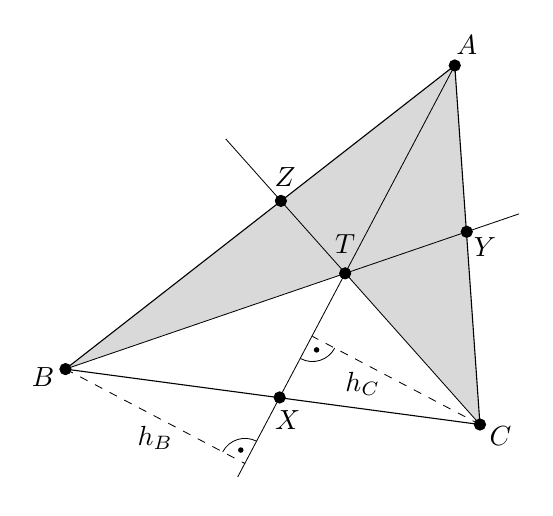
\begin{tikzpicture}[x=0.8cm,y=0.8cm]
		\clip (-4.5,-4.4) rectangle (3.4,2.9);
		\coordinate (A) at (2.28,2.3);
		\coordinate (B) at (-3.9,-2.52);
		\coordinate (C) at (2.68,-3.4);
		\coordinate (T) at (0.54,-1);
		\coordinate (X) at (-0.5,-2.97);
		\coordinate (Y) at (2.47,-0.34);
		\coordinate (Z) at (-0.48,0.15);
		\fill[black!15!white] (A) to (B) to (T) to cycle;
		\fill[black!15!white] (C) to (A) to (T) to cycle;
		\draw (A) to (B);
		\draw (B) to (C);
		\draw (C) to (A);
		\draw[line width=0.3,shorten >=-3.25em] (A) to (X);
		\draw[line width=0.3,shorten >=-2em] (B) to (Y);
		\draw[line width=0.3,shorten >=-3em] (C) to (Z);
		\draw[line width=0.3,dashed] (B) to node[below,pos=0.5] {$h_B$} (-1.05,-4.02) ;
		\draw[line width=0.3,dashed] (C) to node[below,pos=0.7] {$h_C$} (0.02,-2);
		\draw[line width=0.3, shift={(-1.05,-4.02)}] (62.2:0.32cm) arc (62.2:152.2:0.32cm);
		\fill[shift={(-1.05,-4.02)}] (107.2:0.18cm) circle (1pt);
		\draw [line width=0.3,shift={(0.02,-2)}] (-117.8:0.32cm) arc (-117.8:-27.8:0.32cm);
		\fill[shift={(0.02,-2)}] (-72.8:0.18cm) circle (1pt);
		\draw[fill=black] (A) circle (2pt) node[shift={(60:2ex)}] {$A$};
		\draw[fill=black] (B) circle (2pt) node[shift={(200:2ex)}] {$B$};
		\draw[fill=black] (C) circle (2pt) node[shift={(-30:2ex)}] {$C$};
		\draw[fill=black] (T) circle (2pt) node[shift={(90:2.5ex)}] {$T$};
		\draw[fill=black] (X) circle (2pt) node[shift={(-70:2ex)}] {$X$};
		\draw[fill=black] (Y) circle (2pt) node[shift={(-40:2ex)}] {$Y$};
		\draw[fill=black] (Z) circle (2pt) node[shift={(80:2ex)}] {$Z$};
	\end{tikzpicture}
\end{figure}

Es gibt eine Version des Satzes von Ceva, die auch dann gilt, wenn die Punkte $X$,~$Y$ und~$Z$ nicht notwendigerweise im Inneren der Strecken $\overline{BC}$, $\overline{CA}$ und~$\overline{AB}$ liegen. Der größte Teil des Beweises funktioniert auch im allgemeineren Fall, nur das letzte Argument geht schief: Für jede positive reelle Zahl~$\lambda$ (außer $\lambda=1$) gibt es \emph{zwei} Punkte~$X_\lambda$ auf der Geraden~$BC$, für die $\abs{BX_\lambda}/\abs{X_\lambda C}=\lambda$ gilt: einen im Inneren von~$\overline{BC}$ und einen außerhalb. Dieses Problem lässt sich beheben, indem wir \emph{gerichtete Strecken} verwenden. Dafür wählen wir eine Richtung auf der Geraden~$BC$. Für zwei verschiedene Punkte $D$~und~$E$ auf der Geraden~$BC$ ordnen wir der Strecke~$\overline{DE}$ die positive Länge $+\abs{DE}$ oder die negative Länge $-\abs{DE}$ zu, je nachdem, ob $D$~und~$E$ in der gewählten Richtung oder entgegensetzt zur gewählten Richtung auf der Geraden~$BC$ liegen. Die gerichtete Streckenlänge von~$\overline{DE}$ notieren wir einfach als~$DE$ (das kollidiert zwar mit der Bezeichnung für die Gerade~$DE$, aber es wird stets aus dem Kontext klar sein, was gemeint ist). Das Vorzeichen der gerichteten Streckenlängen $BX$ und~$CX$ hängt von der Wahl der Richtung auf~$BC$ ab, nicht aber das Verhältnis $BX/XC$! Wir erhalten, unabhängig von der Wahl der Richtung, dass das Verhältnis $BX/XC$ positiv ist, wenn $X$ im Inneren von~$\overline{BC}$ liegt, und negativ, wenn $X$ außerhalb liegt. Mit gerichteten Streckenlängen gibt es folglich für jede reelle Zahl $\lambda\neq 0,-1$ genau einen Punkt~$X_\lambda$ auf~$BC$ verschieden von $B$ und~$C$, für den $BX_\lambda/X_\lambda C=\lambda$ gilt.

Analog lassen sich \emph{gerichtete Flächeninhalte} definieren: Einem Dreieck $DEF$ ordnen wir den positiven Flächeninhalt $+\mathrm{A}_{DEF}$ oder den negativen Flächeninhalt $-\mathrm{A}_{DEF}$ zu, je nachdem, ob das Dreieck $DEF$ mathematisch positiv oder negativ orientiert ist.

In der allgemeineren Version des Satzes von Ceva tritt leider eine weitere Feinheit auf:
% Tien: Wirklich? "Subtilität"? Wie wäre es mit "Feinheit"?
Es kann passieren, dass die Geraden $AX$, $BY$ und~$CZ$ paarweise parallel sind. Dann schneiden sie sich gewissermaßen \enquote{im Unendlichen} und wir sollten erwarten, dass Gleichung aus dem Satz von Ceva auch in diesem Fall erfüllt ist. Somit erhalten wir den folgenden Satz:

\begin{satzmitnamen}[Gerichteter Satz von Ceva]
	Sei $ABC$ ein Dreieck und seien $X$,~$Y$ und~$Z$ Punkte auf den Geraden $BC$, $CA$ und~$AB$ \embrace{verschieden von $A$,~$B$ und~$C$}. Die Geraden $AX$, $BY$ und~$CZ$ schneiden sich genau dann in einem Punkt oder sind paarweise parallel, wenn die folgende Gleichung \embrace{mit gerichteten Streckenlängen} gilt:
	\begin{equation*}%\label{eq:GerichteterCeva}
		\frac{BX}{XC}\cdot \frac{CY}{YA}\cdot \frac{AZ}{ZB}=1\,.
	\end{equation*}
\end{satzmitnamen}

\begin{proof}
	Wenn die Geraden $AX$, $BY$ und~$CZ$ paarweise parallel sind, folgt die behauptete Gleichung leicht aus dem Strahlensatz (der auch für orientierte Streckenlängen gültig ist). Indem wir den Strahlensatz zuerst auf die Parallelen $AX\parallel BY$ und danach auf die Parallelen $BY\parallel CZ$ anwenden, erhalten wir
	\begin{equation*}
		\frac{BX}{XC}=\frac{BA}{AZ}\quad\text{and}\quad \frac{CY}{YA}=\frac{ZB}{BA}\,.
	\end{equation*}
	Aus diesen beiden Gleichungen folgt sofort die behauptete Gleichung
	\begin{equation*}
		\frac{BX}{XC}\cdot \frac{CY}{YA}\cdot \frac{AZ}{ZB}=\frac{BA}{BA}=1\,.
	\end{equation*}
	
	Wenn sich $AX$, $BY$ und~$CZ$ in einem Punkt~$T$ schneiden, können wir die behauptete Gleichung auf die gleiche Weise wie im Satz von Ceva beweisen, nur dass wir gerichtete Streckenlängen und die gerichteten Flächeninhalte der Dreiecke $ABT$, $BCT$ und $CAT$ verwenden. Die Umkehrung lässt sich ebenfalls völlig analog beweisen.
\end{proof}

Der Satz von Ceva hat auch eine trigonometrische Version, die ebenfalls sehr nützlich sein kann:
\begin{satzmitnamen}[Trigonometrischer Satz von Ceva]
	Sei $ABC$ ein Dreieck und seien $X$,~$Y$ und~$Z$ Punkte auf den Geraden $BC$, $CA$ und~$AB$ \embrace{verschieden von $A$,~$B$ und~$C$}. Die Geraden $AX$, $BY$ und~$CZ$ schneiden sich genau dann in einem Punkt, wenn die folgende Gleichung \embrace{mit gerichteten Winkeln} gilt:
	\begin{equation*}%\label{eq:TrigonometrischerCeva}
		\frac{\sin\winkel BAX}{\sin\winkel XAC}\cdot \frac{\sin \winkel CBY}{\sin\winkel YBA}\cdot \frac{\sin \winkel ACZ}{\sin\winkel ZCB}=1\,.
	\end{equation*}
\end{satzmitnamen}

\begin{proof}
	Übungsaufgabe. (\emph{Tipp: Verwende die Formel $\mathrm{A}_{ABT}=\frac12\abs{AB}\cdot \abs{AT}\cdot \sin\winkel BAT$ und argumentiere dann analog zum Beweis des normalen Satzes von Ceva.})
	% Tien: Den kommentierten Text habe ich Korrektur gelesen.
	%		Wir nehmen zuerst an, dass sich $AX$, $BY$ und~$CZ$ im Punkt~$T$ schneiden. Wie vorher betrachten wir die (gerichteten) Flächeninhalte von $ABT$ und $CAT$. Nach der trigonometrischen Flächeninhaltsformel ist $\mathrm{A}_{ABT}=\frac 12\abs{AB}\cdot \abs{AT}\cdot \sin\winkel BAT$ und $\mathrm{A}_{CAT}=\frac 12\abs{AC}\cdot \abs{AT}\cdot \sin\winkel TAC$. Es gilt $\sin\winkel BAT=\pm\sin\winkel BAX$ und $\sin\winkel TAC=\pm\sin\winkel XAC$, je nachdem, ob $X$ auf der gleichen Seite von~$A$ wie~$T$ liegt oder nicht. In jedem Fall heben sich die Vorzeichen auf und wir erhalten $\sin\winkel BAX/\sin\winkel XAC=\sin\winkel BAT/\sin\winkel TAC$. Folglich gilt
	%		\begin{equation*}
		%			\frac{\sin\winkel BAX}{\sin\winkel XAC}=\frac{\mathrm{A}_{ABT}}{\mathrm{A}_{CAT}}\cdot \frac{\frac12\abs{AC}\cdot\abs{AT}}{\frac12\abs{AB}\cdot \abs{AT}}=\frac{\mathrm{A}_{ABT}}{\mathrm{A}_{CAT}}\cdot \frac{\abs{AC}}{\abs{AB}}
		%		\end{equation*}
	%		Analoge Gleichungen gelten auch für die anderen Winkel. Folglich ist
	%		\begin{equation*}
		%			\frac{\sin\winkel BAX}{\sin\winkel XAC}\cdot \frac{\sin \winkel CBY}{\sin\winkel YBA}\cdot \frac{\sin \winkel ACZ}{\sin\winkel ZCB}=\frac{\mathrm{A}_{ABT}}{\mathrm{A}_{CAT}}\cdot \frac{\abs{AC}}{\abs{AB}}\cdot \frac{\mathrm{A}_{BCT}}{\mathrm{A}_{ABT}}\cdot \frac{\abs{AB}}{\abs{BC}}\cdot \frac{\mathrm{A}_{CAT}}{\mathrm{A}_{BCT}}\cdot \frac{\abs{BC}}{\abs{AC}}=1\,,
		%		\end{equation*}
	%		wie gewünscht. Wenn umgekehrt die gewünschte Gleichung gilt, können wir analog zum Beweis des Satzes von Ceva argumentieren, dass sich $AX$, $BY$ und~$CZ$ in der Tat in einem Punkt schneiden müssen.
\end{proof}

Aus dem Satz von Ceva und seiner trigonometrischen Variante folgen sofort einige klassische Resultate aus der Dreiecksgeometrie.

\begin{aufgabe*}
	Benutze den Satz von Ceva oder seine trigonometrische Version, um zu zeigen, dass sich in jedem Dreieck die Seitenhalbierenden, die Winkelhalbierenden und die Höhen jeweils in einem Punkt schneiden!
\end{aufgabe*}

\begin{aufgabe*}
	Sei $ABC$ ein Dreieck und seien $D$,~$E$ und~$F$ die Berührpunkt des Inkreises mit $\overline{BC}$, $\overline{CA}$ und~$\overline{AB}$. Beweise, dass sich die Geraden $AD$, $BE$ und~$CF$ in einem Punkt schneiden \embrace{dieser Punkt ist der sogenannte \emph{Gergonnepunkt} von $ABC$}.
\end{aufgabe*}

\subsection*{Der Satz von Menelaos}
\begin{satzmitnamen}[Satz von Menelaos]
	Sei $ABC$ ein Dreieck und seien $X$,~$Y$ und~$Z$ Punkte auf den Geraden $BC$, $CA$ und~$AB$ \embrace{verschieden von $A$,~$B$ und~$C$}. Dann liegen die Punkte $X$,~$Y$ und~$Z$ genau dann auf einer Geraden, wenn die folgende Gleichung \embrace{mit gerichteten Streckenlängen} gilt:
	\begin{equation*}%\label{eq:GerichteterMenelaos}
		\frac{BX}{XC}\cdot \frac{CY}{YA}\cdot \frac{AZ}{ZB}=-1\,.
	\end{equation*}
\end{satzmitnamen}

\begin{proof}
	Nehmen wir zunächst an, dass $X$,~$Y$ und~$Z$ auf einer Geraden~$\ell$ liegen. Sei $H_A$ der Lotfußpunkt von~$A$ auf~$\ell$ und definiere $H_B$,~$H_C$ analog. Die Höhen von $B$~und~$C$ auf~$\ell$ sind parallel. Aus dem Strahlensatz (der in dieser Form auch für gerichtete Streckenlängen gültig ist) erhalten wir also $BX/XC=BH_B/H_CC=-BH_B/CH_C$. Analoge Gleichungen gelten für $CY/YA$ und $AZ/ZB$. Es folgt
	\begin{equation*}
		\frac{BX}{XC}\cdot \frac{CY}{YA}\cdot \frac{AZ}{ZB}=\parens*{-\frac{BH_B}{CH_C}}\parens*{-\frac{CH_C}{AH_A}}\parens*{-\frac{AH_A}{BH_B}}=-1\,,
	\end{equation*}
	wie gewünscht. Wenn umgekehrt die Gleichung aus dem Satz von Menelaos gilt, können wir wie im Beweis des Satzes von Ceva argumentieren: Sei $X'$ derjenige Punkt auf~$BC$, für den $X'$,~$Y$ und~$Z$ kollinear sind. Wir müssen $X=X'$ zeigen. Wie wir gerade gesehen haben, ist für den Punkt~$X'$ ebenfalls die Gleichung aus dem Satz von Menelaos erfüllt. Es muss also $BX/XC=BX'/X'C$ gelten. Für jede reelle Zahl $\lambda\neq 0$ gibt es aber genau einen Punkt~$X_\lambda$ auf der Geraden~$BC$, für den $BX_\lambda/X_\lambda C=\lambda$ gilt. Folglich muss in der Tat $X=X'$ sein.
\end{proof}

\begin{center}
	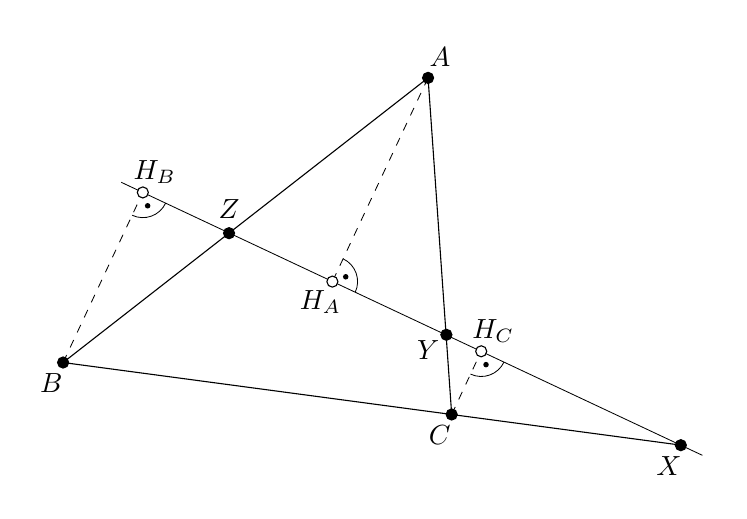
\begin{tikzpicture}[x=0.75cm,y=0.75cm]
		\clip (-4.5,-4.7) rectangle (7.2,3.15);
		\coordinate (A) at (2.28,2.3);
		\coordinate (B) at (-3.9,-2.52);
		\coordinate (C) at (2.68,-3.4);
		\coordinate (Y) at (2.59,-2.05);
		\coordinate (X) at (6.56,-3.92);
		\coordinate (Z) at (-1.09,-0.33);
		\coordinate (HA) at (0.66,-1.15);
		\coordinate (HB) at (-2.55,0.36);
		\coordinate (HC) at (3.18,-2.33);
		\draw (A) to (B);
		\draw[shorten >=-8.5em] (B) to (C); % Tien: Ich habe die Gerade mal etwas länger gemacht (davor war das -6.5em)
		\draw[line width=0.3, dashed] (A) to (HA);
		\draw[line width=0.3, dashed] (B) to (HB);
		\draw[line width=0.3, dashed] (C) to (HC);
		\draw (C) to (A);
		\draw[line width=0.3,shorten <=-2ex,shorten >=-2ex] (HB) to (X);
		\draw[line width=0.3,shift={(HB)}] (-115.15:0.32cm) arc (-115.15:-25.15:0.32cm);
		\fill[shift={(HB)}] (-70.15:0.18cm) circle (1pt);
		\draw[line width=0.3,shift={(HA)}] (-25.15:0.32cm) arc (-25.15:64.85:0.32cm);
		\fill[shift={(HA)}] (19.85:0.18cm) circle (1pt);
		\draw[line width=0.3,shift={(HC)}] (-115.15:0.32cm) arc (-115.15:-25.15:0.32cm);
		\fill[shift={(HC)}] (-70.15:0.18cm) circle (1pt);
		\draw[fill=black] (A) circle (2pt) node[shift={(60:2ex)}] {$A$};
		\draw[fill=black] (B) circle (2pt) node[shift={(240:2ex)}] {$B$};
		\draw[fill=black] (C) circle (2pt) node[shift={(240:2ex)}] {$C$};
		\draw[fill=black] (X) circle (2pt) node[shift={(240:2ex)}] {$X$};
		\draw[fill=black] (Y) circle (2pt) node[shift={(220:2ex)}] {$Y$};
		\draw[fill=black] (Z) circle (2pt) node[shift={(90:2ex)}] {$Z$};
		\draw[fill=white] (HA) circle (2pt) node[shift={(240:2ex)}] {$H_A$};
		\draw[fill=white] (HB) circle (2pt) node[shift={(60:2ex)}] {$H_B$};
		\draw[fill=white] (HC) circle (2pt) node[shift={(60:2ex)}] {$H_C$};
	\end{tikzpicture}
	% Tien: Was macht das hier? Wenn du unbedingt willst, dass das Bild auf derselben Seite passen soll, dann solltest du am besten auf die figure Umgebung verzichten (der Zweck ist automatisches Setzen von Floats).
	% Vielleicht willst du \begin{center}...\end{center} verwenden?
	%\vspace{-2em}
\end{center}

\subsection*{Weitere Übungsaufgaben}
\begin{aufgabe*}
	Sei $ABC$ ein Dreieck und sei $P$ ein Punkt verschieden von $A$,~$B$ und~$C$. Sei $\ell_A$ das Spiegelbild der Geraden~$AP$ an der Winkelhalbierenden von $\winkel BAC$ und definiere $\ell_B$,~$\ell_C$ analog. Zeige, dass sich die Geraden $\ell_A$,~$\ell_B$ und~$\ell_C$ in einem Punkt schneiden \embrace{dieser Schnittpunkt wird der \emph{zu~$P$ isogonal konjugierte Punkt} genannt}.
\end{aufgabe*}

\begin{aufgabe*}
	Sei $ABC$ ein Dreieck und sei $P$ ein Punkt auf dem Umkreis $\odot ABC$. Ferner seien $P_a$,~$P_b$ und~$P_c$ die Lotfußpunkte von~$P$ auf die Geraden $BC$, $CA$ und~$AB$. Zeige, dass die Punkte $P_a$, $P_b$ und~$P_c$ auf einer Geraden liegen \embrace{diese Gerade wird üblicherweise \emph{Simson-Gerade} genannt}.
\end{aufgabe*}

\begin{aufgabe*}
	Sei $ABCD$ ein Tangentenviereck. Der Inkreis~$\omega$ berühre die Seiten $\overline{AB}$, $\overline{BC}$, $\overline{CD}$ und~$\overline{DA}$ in den Punkten $W$,~$X$, $Y$ und~$Z$. Zeige, dass sich die Geraden $WX$, $YZ$ und~$AC$ in einem Punkt schneiden oder paarweise parallel sind.
\end{aufgabe*}

\begin{aufgabe*}
	% Tien: Lol, ist das eine Shortlist?
	Für ein konvexes Fünfeck $ABCDE$ gelte $\winkel BAC=\winkel CAD=\winkel DAE$ sowie $\winkel CBA=\winkel DCA=\winkel EDA$. Der Schnittpunkt der Diagonalen $BD$ und~$CE$ wird mit~$P$ bezeichnet. Beweise, dass die Gerade~$AP$ durch den Mittelpunkt der Seite~$\overline{CD}$ verläuft.
\end{aufgabe*}

\begin{aufgabe*}
	Sei $ABC$ ein spitzwinkliges Dreieck mit $\abs{BC}>\abs{CA}$. Die Mittelsenkrechte der Strecke~$\overline{AB}$ schneide die Gerade~$BC$ in~$P$ und die Gerade~$CA$ in~$Q$. Sei $R$ der Lotfußpunkt von~$R$ auf~$CA$ und $S$ der Lotfußpunkt von~$Q$ auf~$BC$. Zeige, dass $R$,~$S$ und der Mittelpunkt der Strecke~$\overline{AB}$ auf einer Geraden liegen. 
\end{aufgabe*}

\begin{aufgabe*}[*]
	Sei $ABC$ ein Dreieck mit Inkreismittelpunkt~$I$ und sei $\omega$ ein Kreis mit Mittelpunkt~$I$ im Inneren des Dreiecks. Die Lote von~$I$ auf die Dreiecksseiten $BC$, $CA$ und~$AB$ schneiden~$\omega$ in $A'$,~$B'$ und~$C'$. Zeige, dass sich die Geraden $AA'$, $BB'$ und~$CC'$ in einem Punkt schneiden.
\end{aufgabe*}

\begin{aufgabe*}[***]
	Beweise den Satz von Pascal:
	\begin{satzmitnamen}[Satz von Pascal]
		Sei $ABCDEF$ ein Sehnensechseck, dessen gegenüberliegende Seiten paarweise nicht-parallel sind. Die Seiten $AB$~und~$DE$ schneiden sich in~$X$, die Seiten $BC$~und~$EF$ schneiden sich in~$Y$ und die Seiten $CD$~und~$FA$ schneiden sich in~$Z$. Dann sind $X$,~$Y$ und~$Z$ kollinear.
	\end{satzmitnamen}
\end{aufgabe*}